\documentclass[conference]{IEEEtran}
%\IEEEoverridecommandlockouts
% The preceding line is only needed to identify funding in the first footnote. If that is unneeded, please comment it out.
\usepackage{cite}
\usepackage{amsmath,amssymb,amsfonts}
\usepackage{algorithmic}
\usepackage{graphicx}
\graphicspath{{images/}}
\usepackage{textcomp}
\usepackage{xcolor}
\usepackage{url}
\usepackage[hidelinks]{hyperref}
\def\BibTeX{{\rm B\kern-.05em{\sc i\kern-.025em b}\kern-.08em
    T\kern-.1667em\lower.7ex\hbox{E}\kern-.125emX}}
\begin{document}

\title{Learning Relative Interactions through Imitation \\ \vspace{0.5\baselineskip}
{
	\large {Università della Svizzera Italiana}\\
	{Faculty of Informatics} \\
	Lugano, Switzerland \\
	\textit{Project for the Robotics course 2019--2020}\\
}
%\thanks{Identify applicable funding agency here. If none, delete this.}
}

\author{\IEEEauthorblockN{Giorgia Adorni}
\IEEEauthorblockA{(giorgia.adorni@usi.ch)}
\and
\IEEEauthorblockN{Elia Cereda}
\IEEEauthorblockA{(elia.cereda@usi.ch)}}

\maketitle
\thispagestyle{plain}
\pagestyle{plain}

\begin{abstract}
In this project we trained a neural network to perform specific interactions 
between a robot and objects in the environment, through imitation learning. In 
particular, we tackle the task of moving the robot to a fixed pose with respect 
to a certain object and later extend our method to handle any arbitrary pose 
around this object.

We show that a simple network, with relatively little training data, is able to 
reach very good performance on the fixed-pose task, while more work is needed 
to perform the arbitrary-pose task satisfactorily. We also explore the effect 
of ambiguities in the sensor readings, in particular caused by symmetries in 
the target object, on the behaviour of the learned controller.

\emph{External Resources}---source code~\cite{github}, pitch 
presentation~\cite{pitch} and final presentation~\cite{final-pitch}.

\end{abstract}

%\begin{IEEEkeywords}
%component, formatting, style, styling, insert
%\end{IEEEkeywords}

\section{Introduction}

In robotics, some tasks are relatively easy to perform with complete knowledge 
of the environment, but become more challenging when the environment is only 
partially observable using a robot's sensors. Imitation learning deals with 
this problem by recording the trajectories of an omniscient controller 
performing the desired task, then training a machine learning model to 
replicate them using just the data from the sensors. As such, the machine 
learning model must learn how to extract the relevant information from the data 
it receives, sidestepping the difficulty of implementing the perception part 
manually.

The target platform we choose for our project is the 
marXbot~\cite{bonani2010marxbot}, a research robot originally designed to study 
collective and swarm robotics. The main characteristic making the marXbot 
interesting for this project is its rotating laser scanner, which perceives 
distances and colours of the objects surrounding the robot.

The experiments are run in Enki~\cite{enki}, a high-performance open-source 
simulator for planar robots, which provides collision detection and limited 
physics support for robots evolving on a flat surface. Moreover, it can 
simulate groups of robots hundreds of times faster than real-time.

\begin{figure}[htbp]
	\centerline{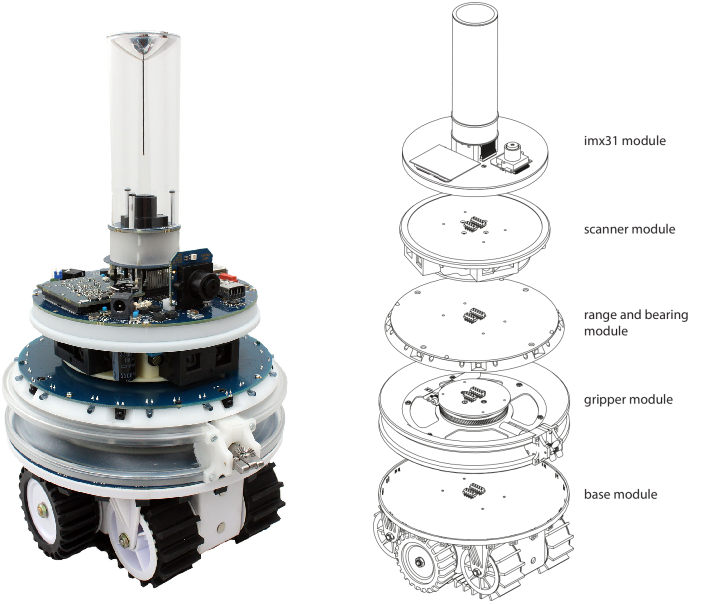
\includegraphics[width=.8\columnwidth]{introduction/marxbot}}
	\caption{Actual image and exploded CAD view of a marXbot.}
	\label{fig:marxbot}
\end{figure}

The task that we 

%The main objective of this project is learning to perform specific 
%interactions between the robot and objects in the 
%environment.
%Write an omniscient controller that performs the desired interaction with 
%complete knowledge of the environment (e.g. 
%position the robot at a certain location relative to an object) using Enki.
%Generate a dataset of simulation runs through Enki. 
%Through imitation learning, train an end-to-end neural network that receives 
%as inputs the sensor distances and the 
%camera image readings and produces commands for the motors that are the left 
%and the right wheel target speeds.
%Evaluate the model trained using Enki.
% 

\section{Controllers}

In an imitation learning setting, there are two controllers involved: an \emph{omniscient} controller, which performs the desired task with perfect knowledge of the environment, and a \emph{learned} controller, which is trained to imitate the behaviour of the omniscient controller.

\subsection{Omniscient controller}

We implemented a controller from the literature that simultaneously controls position and orientation of the robot toward a certain goal pose~\cite{park2011smooth}.

We chose this particular controller because it promised smooth and intuitive 
trajectories, which globally converge to arbitrary goal poses without 
singularities, from any initial pose. Furthermore, this specific formulation 
makes it easy to impose limits on the velocity, acceleration and jerk of the 
resulting paths, ensuring that they would be physically realizable if executed
on a real robot.

The control law is described in an egocentric polar coordinate system, relative to the current pose of the robot. The control variables are the linear $v$ and angular $\omega$ velocities. Given a target pose $T$, the state of the robot is expressed as the triple $(r, \theta, \delta)$, where $r$ is the Euclidean distance from the target position; $\theta \in (-\pi, \pi]$ the target orientation with respect to the line of sight from the robot to the target position; $\delta \in (-\pi, \pi]$ the vehicle orientation with respect to the line of sight, as shown in Figure~\ref{fig:egocentric-coordinates}.

It can be seen that $(r, \theta)$ completely identify the position of the robot, while $\delta$ identifies its orientation. In this formulation, moving the robot to the target pose corresponds to bringing the state to the origin, $(r, \theta, \delta) = (0, 0, 0)$.

\begin{figure}[htbp]
	\centerline{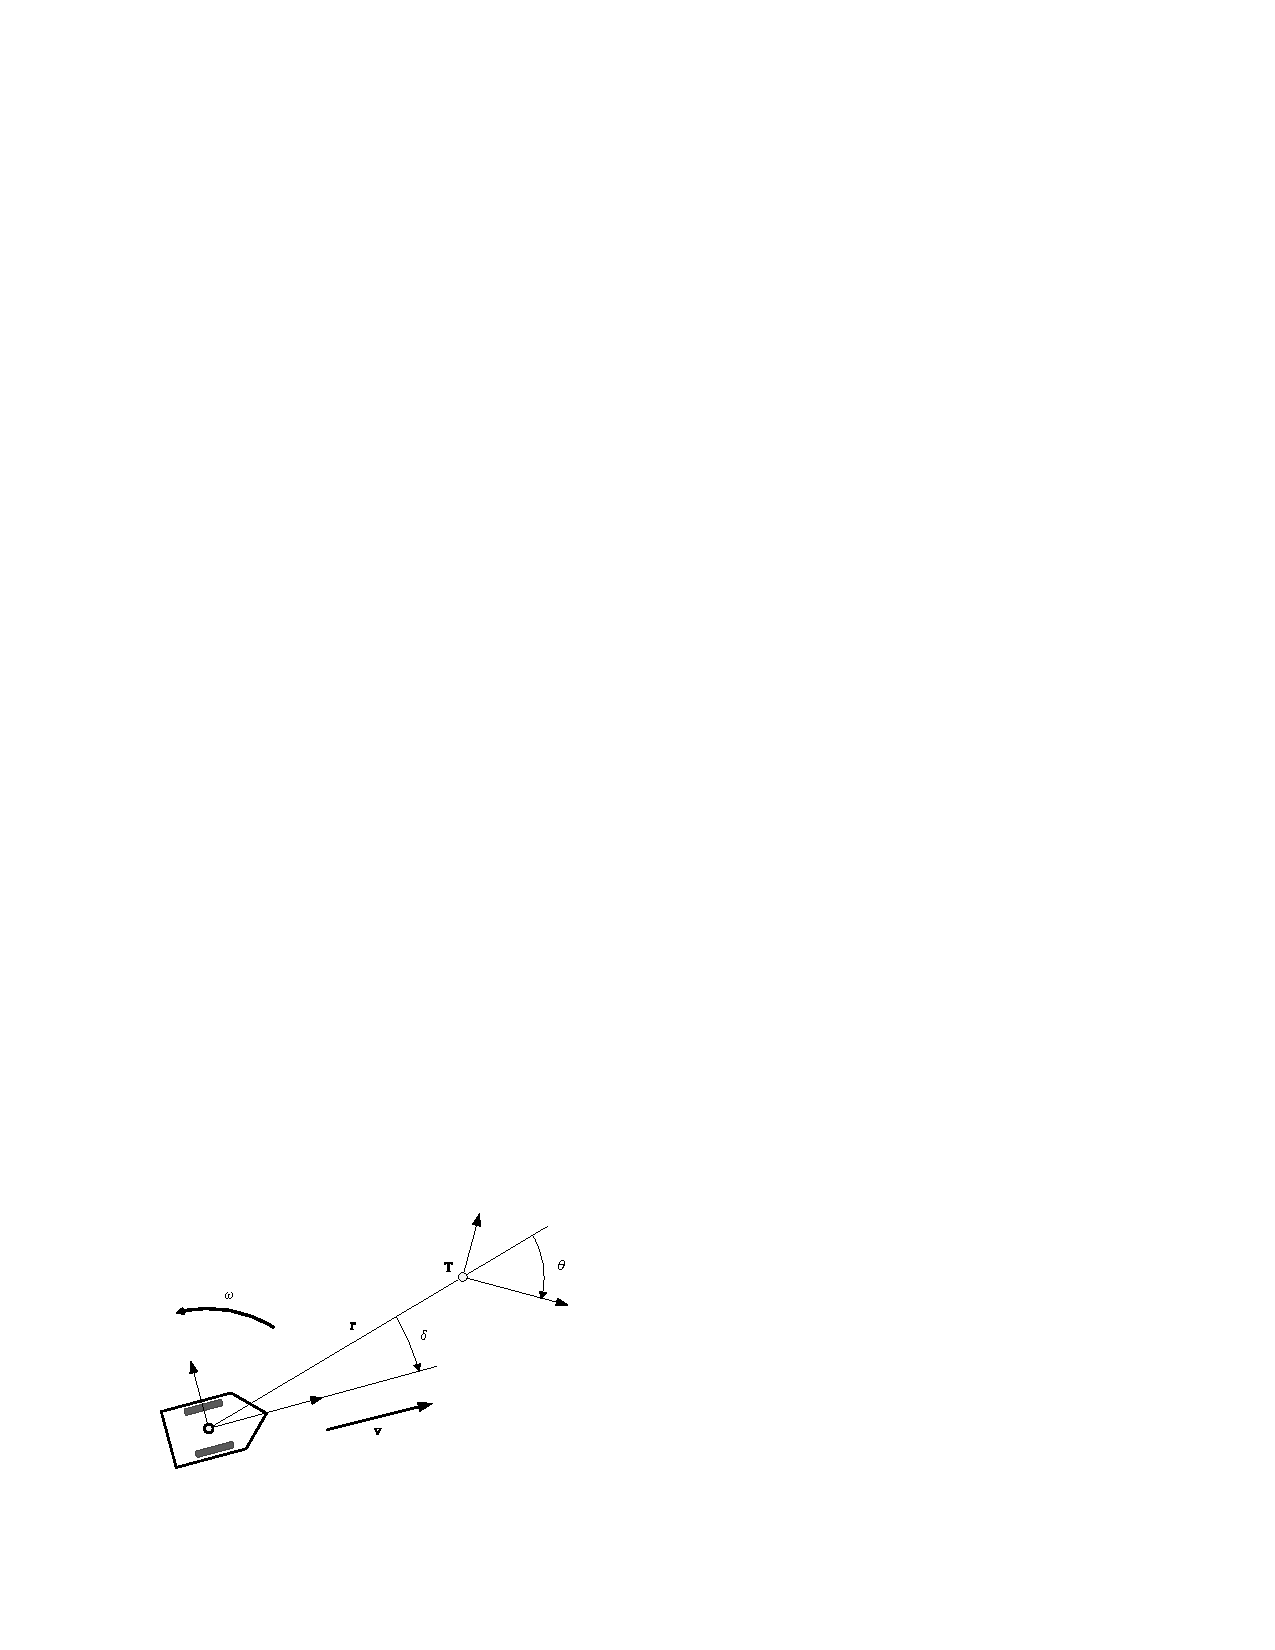
\includegraphics[width=\columnwidth]{controller/egocentric-coordinates}}
	\caption{Egocentric polar coordinate system, relative to the current pose of the robot.}
	\label{fig:egocentric-coordinates}
\end{figure}

Assuming initially the linear velocity $v$ is nonzero positive and given (although not constant), the authors show that the angular velocity $\omega$ only influences $\delta$ directly, which in turn influences $(r, \theta)$. As such, the control problem is decomposed in a slow and a fast subsystem.

The slow subsystem first computes a reference orientation $\hat{\delta}$ to steer the robot toward the origin:
\begin{IEEEeqnarray}{l}
	\hat{\delta} = \arctan(-k_1 \theta)
\end{IEEEeqnarray}

The fast subsystem then controls the angular velocity $\omega$ to bring the current orientation $\delta$ toward the reference orientation $\hat{\delta}$ computed by the slow subsystem (somewhat confusingly, the original paper uses $\delta$ for both the current and reference orientations):
\begin{IEEEeqnarray}{l}
	\omega = -\frac{v}{r} [
		k_2 (\delta - \underbrace{\arctan(-k_1 \theta)}_{\hat{\delta}}) +
		(1 + \underbrace{\frac{k_1}{1 + (k_1\theta)^2}}_{-\dot{\hat{\delta}}})\sin\theta
	] \notag \\
	\label{eq:angular-vel}
\end{IEEEeqnarray}

It can be seen from \eqref{eq:angular-vel} that there is a linear relation between $v$ and $\omega$. In particular, $\, \omega = \kappa(r, \theta, \delta) \, v$ where $\kappa$ is the curvature of the resulting path. It is possible to rewrite \eqref{eq:angular-vel}, such that
\begin{IEEEeqnarray}{l}
	\kappa = -\frac{1}{r} [k_2 (\delta - \hat{\delta}) + (1 - \dot{\hat{\delta}})\sin\theta]
	\label{eq:curvature}
\end{IEEEeqnarray}
which implies that the shape of the path does not depend on the choice of $v$. To ensure a smooth and comfortable trajectory, the authors suggest to choose $v$ so that $v \rightarrow 0$ as $\kappa \rightarrow \pm\infty$ and $v \rightarrow v_\text{max}$ as $\kappa \rightarrow 0$:
\begin{IEEEeqnarray}{l}
	v = \frac{v_\text{max}}{1 + \beta |\kappa(r, \theta, \delta)|^\lambda}
	\label{eq:linear-vel}
\end{IEEEeqnarray}

As written, the control law has a singularity as $r \rightarrow 0$, in other words when the robot approaches the target. We address this problem as suggested in the original paper, by setting $v = k_3 r$ in the neighbourhood of $r = 0$:
\begin{IEEEeqnarray}{l}
	v' = \min(v, k_3 r)
	\label{eq:final-linear-vel}
\end{IEEEeqnarray}

In the equations above $k_1 > 0$, $k_2 > 0$, $k_3 > 0$, $\beta > 0$ and $\lambda > 1$ are design parameters. Figure~\ref{fig:omniscient-trajectories} shows some trajectories generated by this controller, obtained with parameters $k_1 = 1$, $k_2 = 3$, $k_3 = 2$, $\beta = 0.4$ and $\lambda = 2$.

\begin{figure}[htbp]
	\centerline{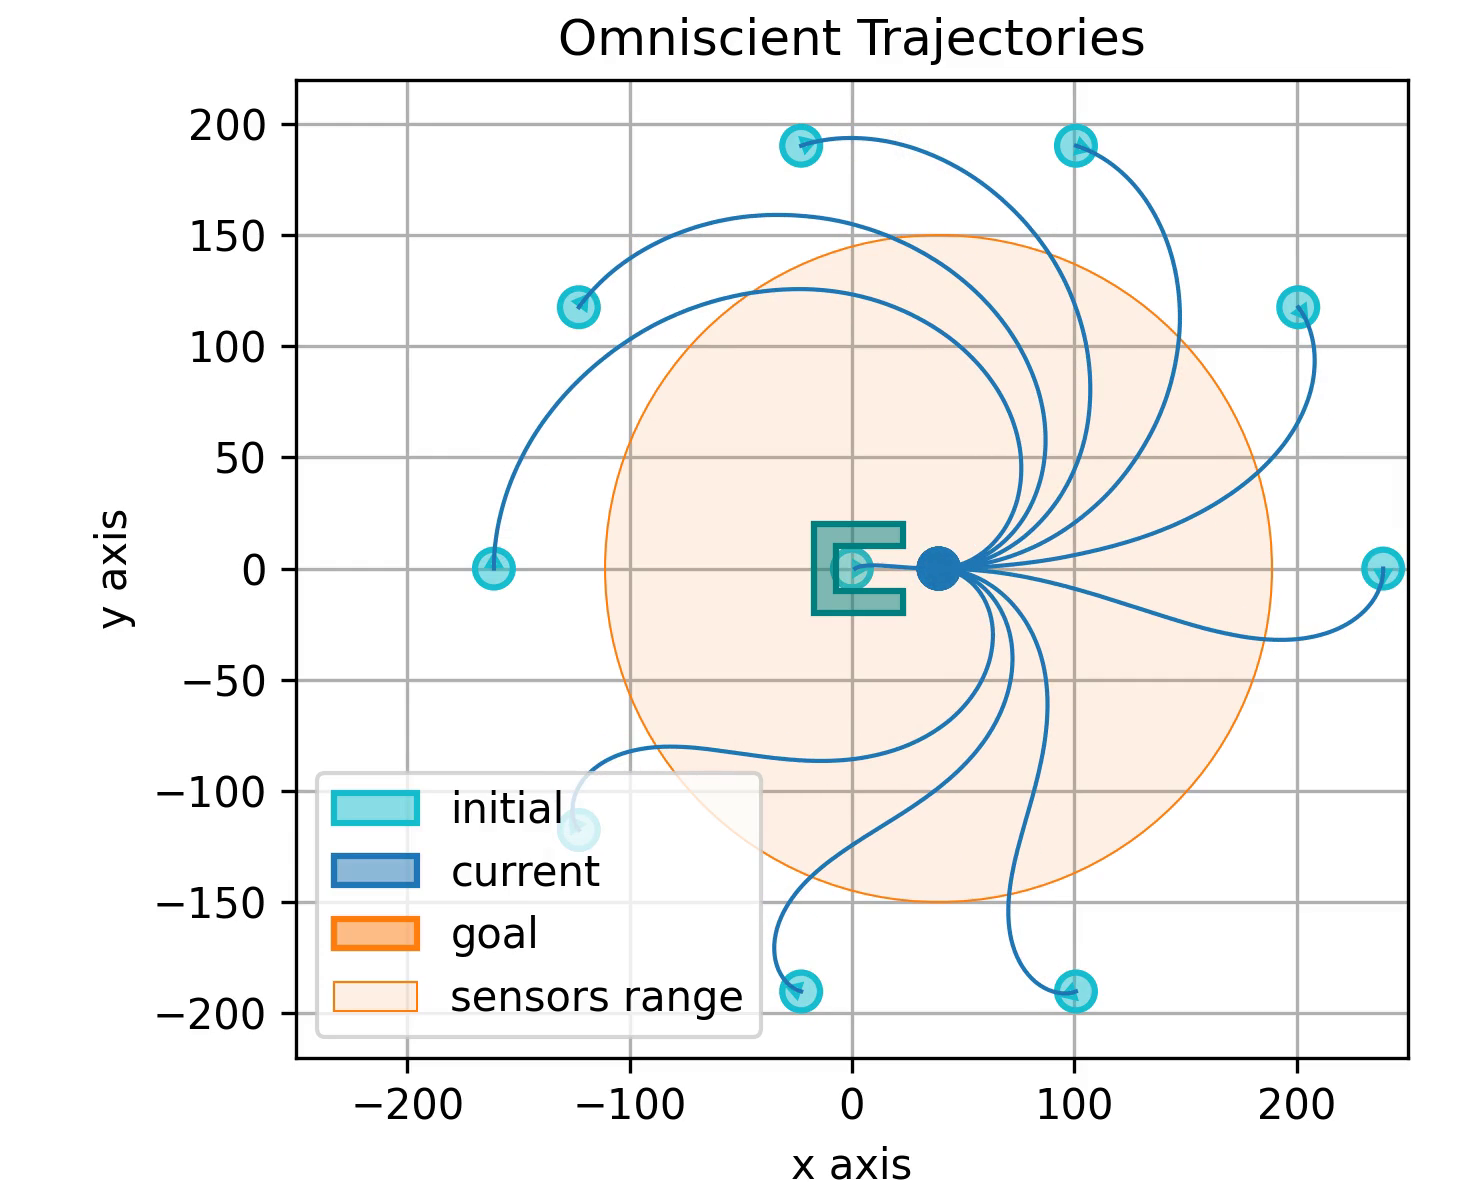
\includegraphics[width=.8\columnwidth]{controller/demo-circle-omniscient-trajectories}}
	\caption{Trajectories of the omniscient controller from 9 initial poses.}
	\label{fig:omniscient-trajectories}
\end{figure}

Finally, we implemented support for reverse gear as suggested by the authors: by simultaneously flipping the orientation of both the robot and the target when $v$ is negative. 

We use the reverse gear to teach the learned controller how to behave when it overshoots the target. This normally never happened with the omniscient controller, so the neural network wouldn't know what to do if it didn't stop precisely over the goal. We used an augmentation technique to ensure that this situation would be present in the training set: we made the robot move in reverse if its initial position was inside a region in front of the goal (i.e. between the arms of the object in Figure~\ref{fig:omniscient-trajectories}).

\subsection{Learned controller}

FIXME


\section{Task 1}
\label{sec:task1}
\subsection{Data Generation Through Enki Simulations}
Relying on Enki and on the omniscient controller, a dataset of 2000 simulation 
runs is generated. 
Each run sets up a world containing:
\begin{itemize}
	\item a \emph{horseshoe-shaped object}, that represents a hypothetical 
	docking 
	station, always at pose $(x=0, y=0, \theta=0)$;
	\item a \emph{fixed goal pose}, in front of the two arms of the object;
	\item a \emph{marXbot}, at a random uniform position and orientation 
	around the 
	goal, up to a maximum distance of 2 meters --- slightly more that the range 
	of the distance sensors.\\
\end{itemize}

A simulation run is stopped either 1 second (10 timesteps) after the robot 
reaches the target pose*, or after 20 seconds (200 timesteps). This ensures 
enough timesteps in which the robot is stopped at the goal, improving 
the performance of the network. The marXbot is considered at target if position 
distance is less than 1 millimetre and orientation less than 0.5 degree.
\\

An hypothetical simulation run results in these distribution of positions at 
the beginning and end of each run, shown 
in Figure \ref{fig:initial-final-positions-omniscient} and in trajectories like 
those shown in Figure 
\ref{fig:trajectories-omniscient}.
%
%\begin{figure}[htbp]
%\centerline{\includegraphics[width=\columnwidth]{dataset/monochromatic-omniscient/initial-final-positions}}
%	\caption{Initial and final positions.}
%	\label{fig:initial-final-positions-omniscient}
%\end{figure}
%
%\begin{figure}[htbp]
%\centerline{\includegraphics[width=.8\columnwidth]{dataset/monochromatic-omniscient/10-robot-trajectories}}
%	\caption{Trajectories of ten randomly selected runs.}
%	\label{fig:trajectories-omniscient}
%\end{figure}

The density of samples in each position can be seen in Figure 
\ref{fig:densisy-omniscient} while the histogram of the time needed to reach 
the goal is shown in Figure \ref{fig:goal-reached-omniscient}. In this case, 
all the runs terminate at the goal.\\

%\begin{figure}[htbp]
%\centerline{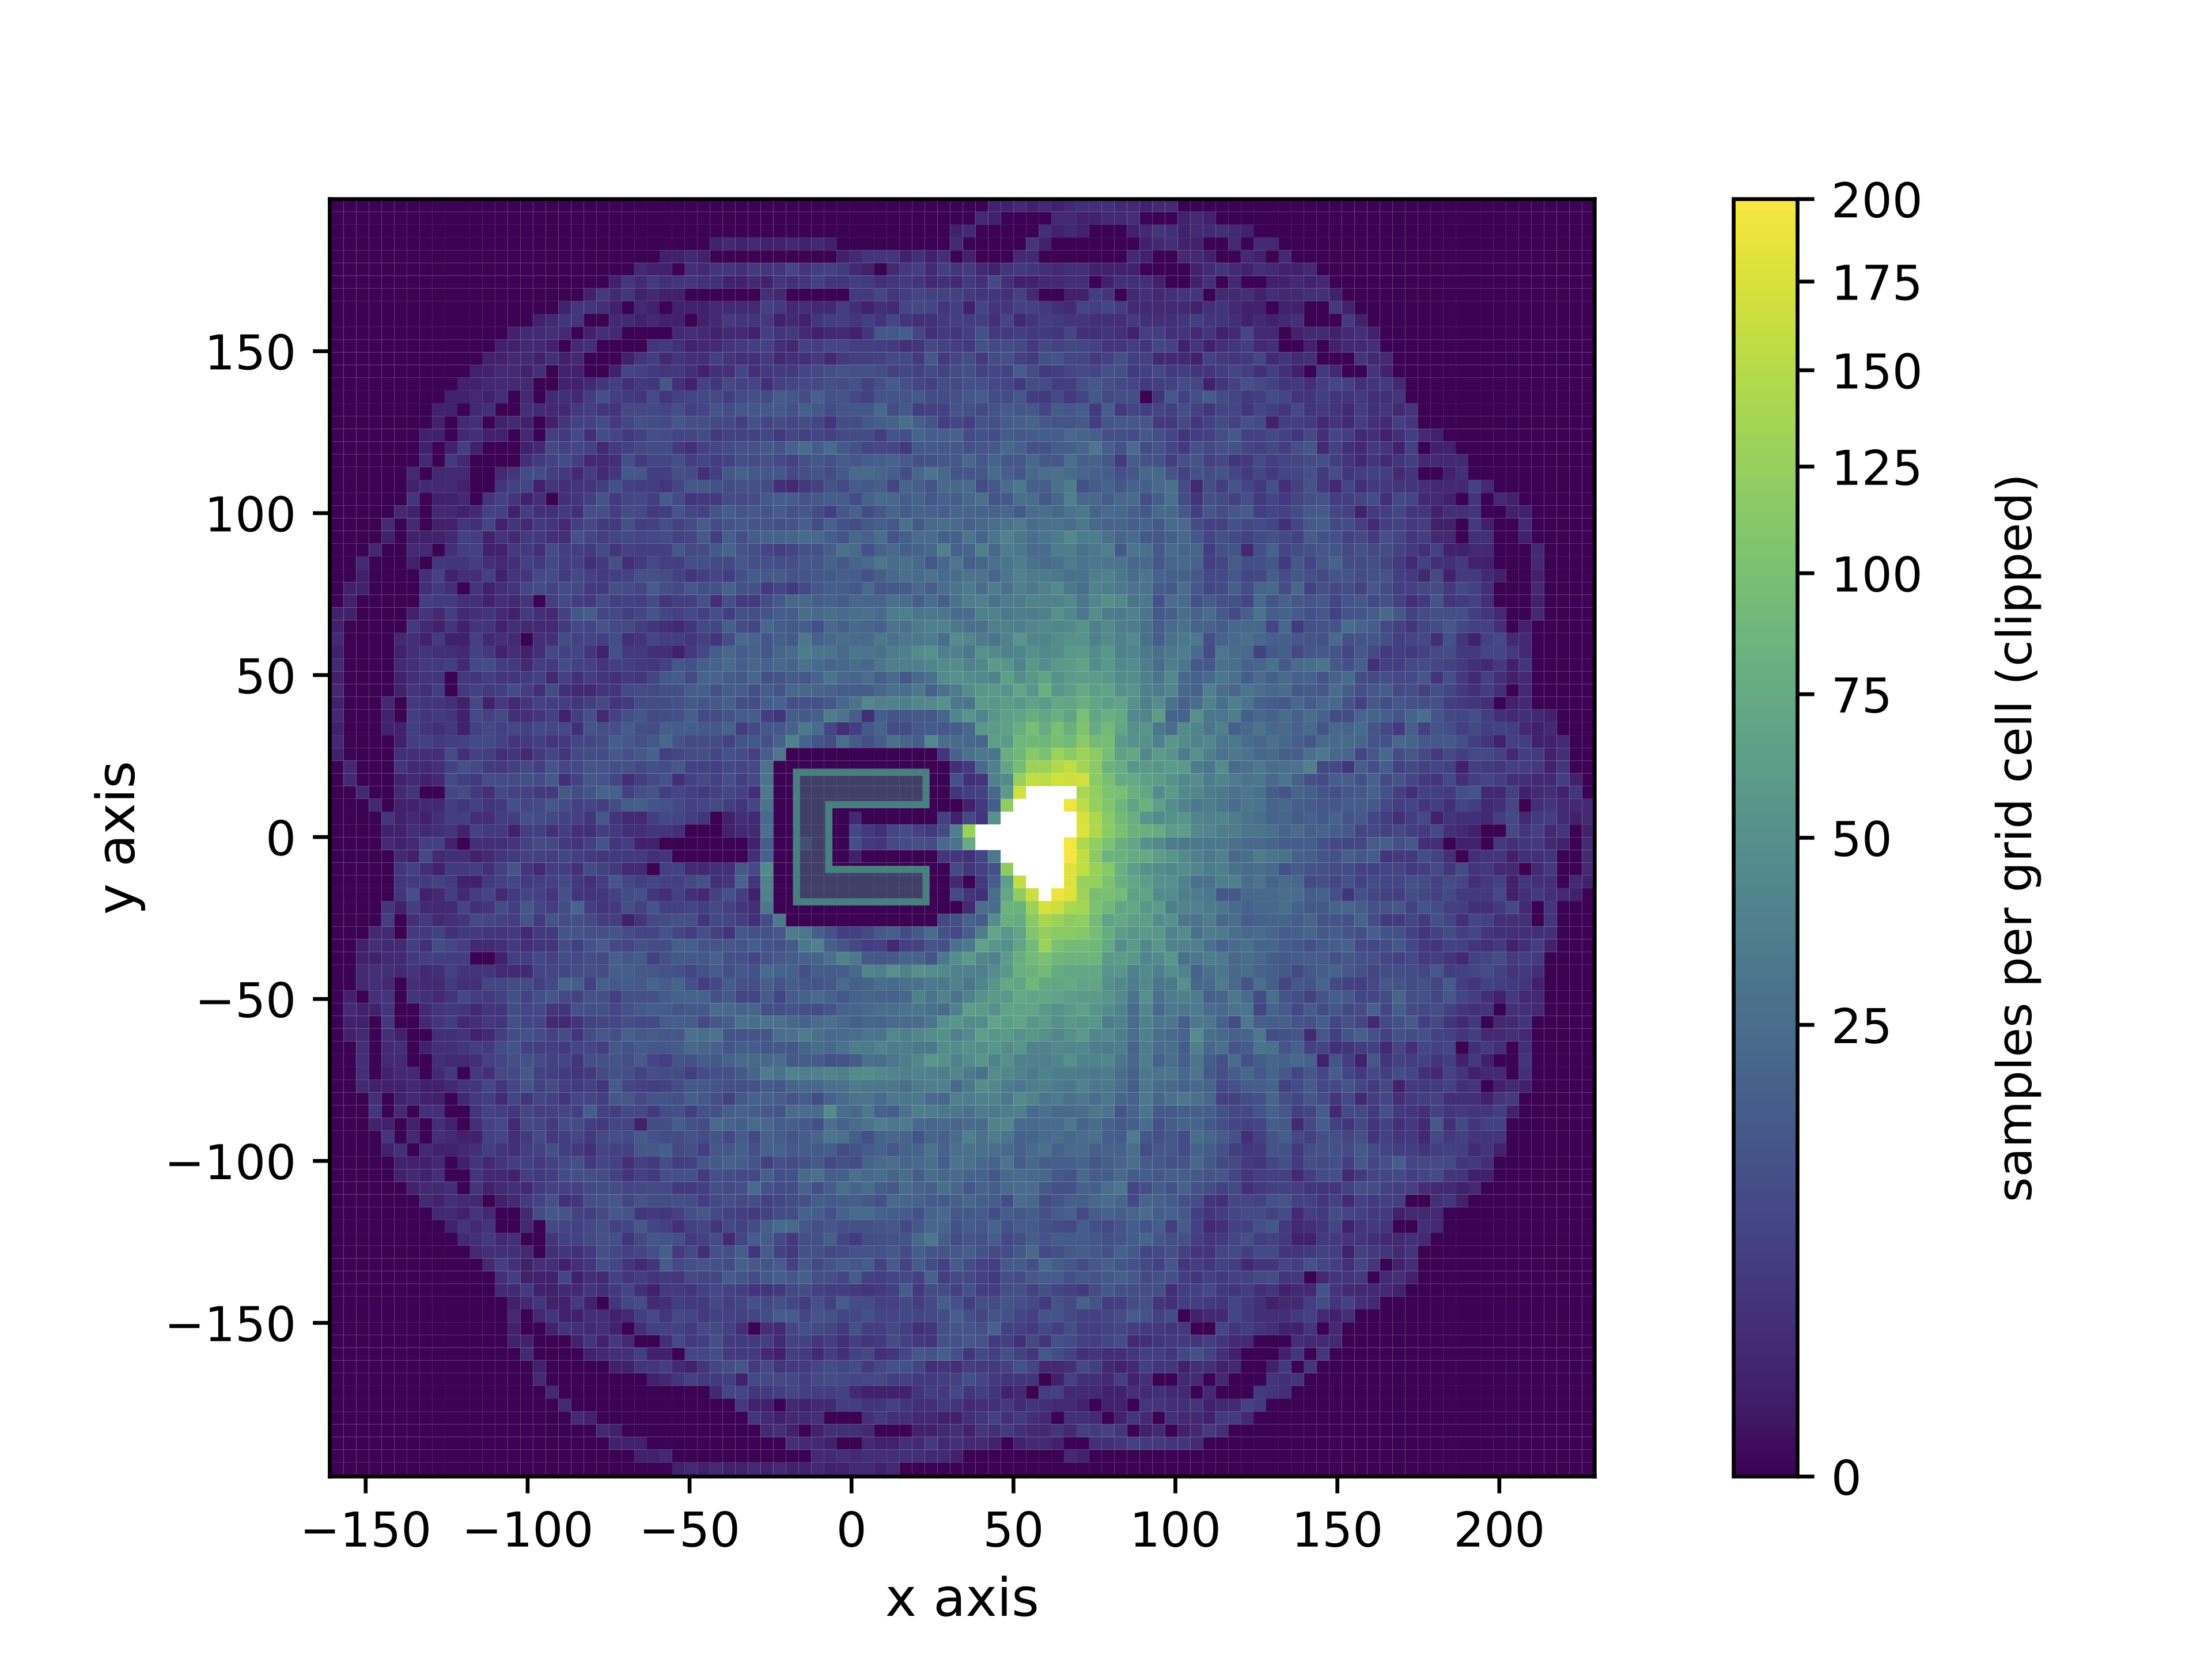
\includegraphics[width=.8\columnwidth]{dataset/monochromatic-omniscient/positions-heatmap}}
%	\caption{Positions heatmap.}
%	\label{fig:densisy-omniscient}
%\end{figure}
%
%
%\begin{figure}[htbp]
%\centerline{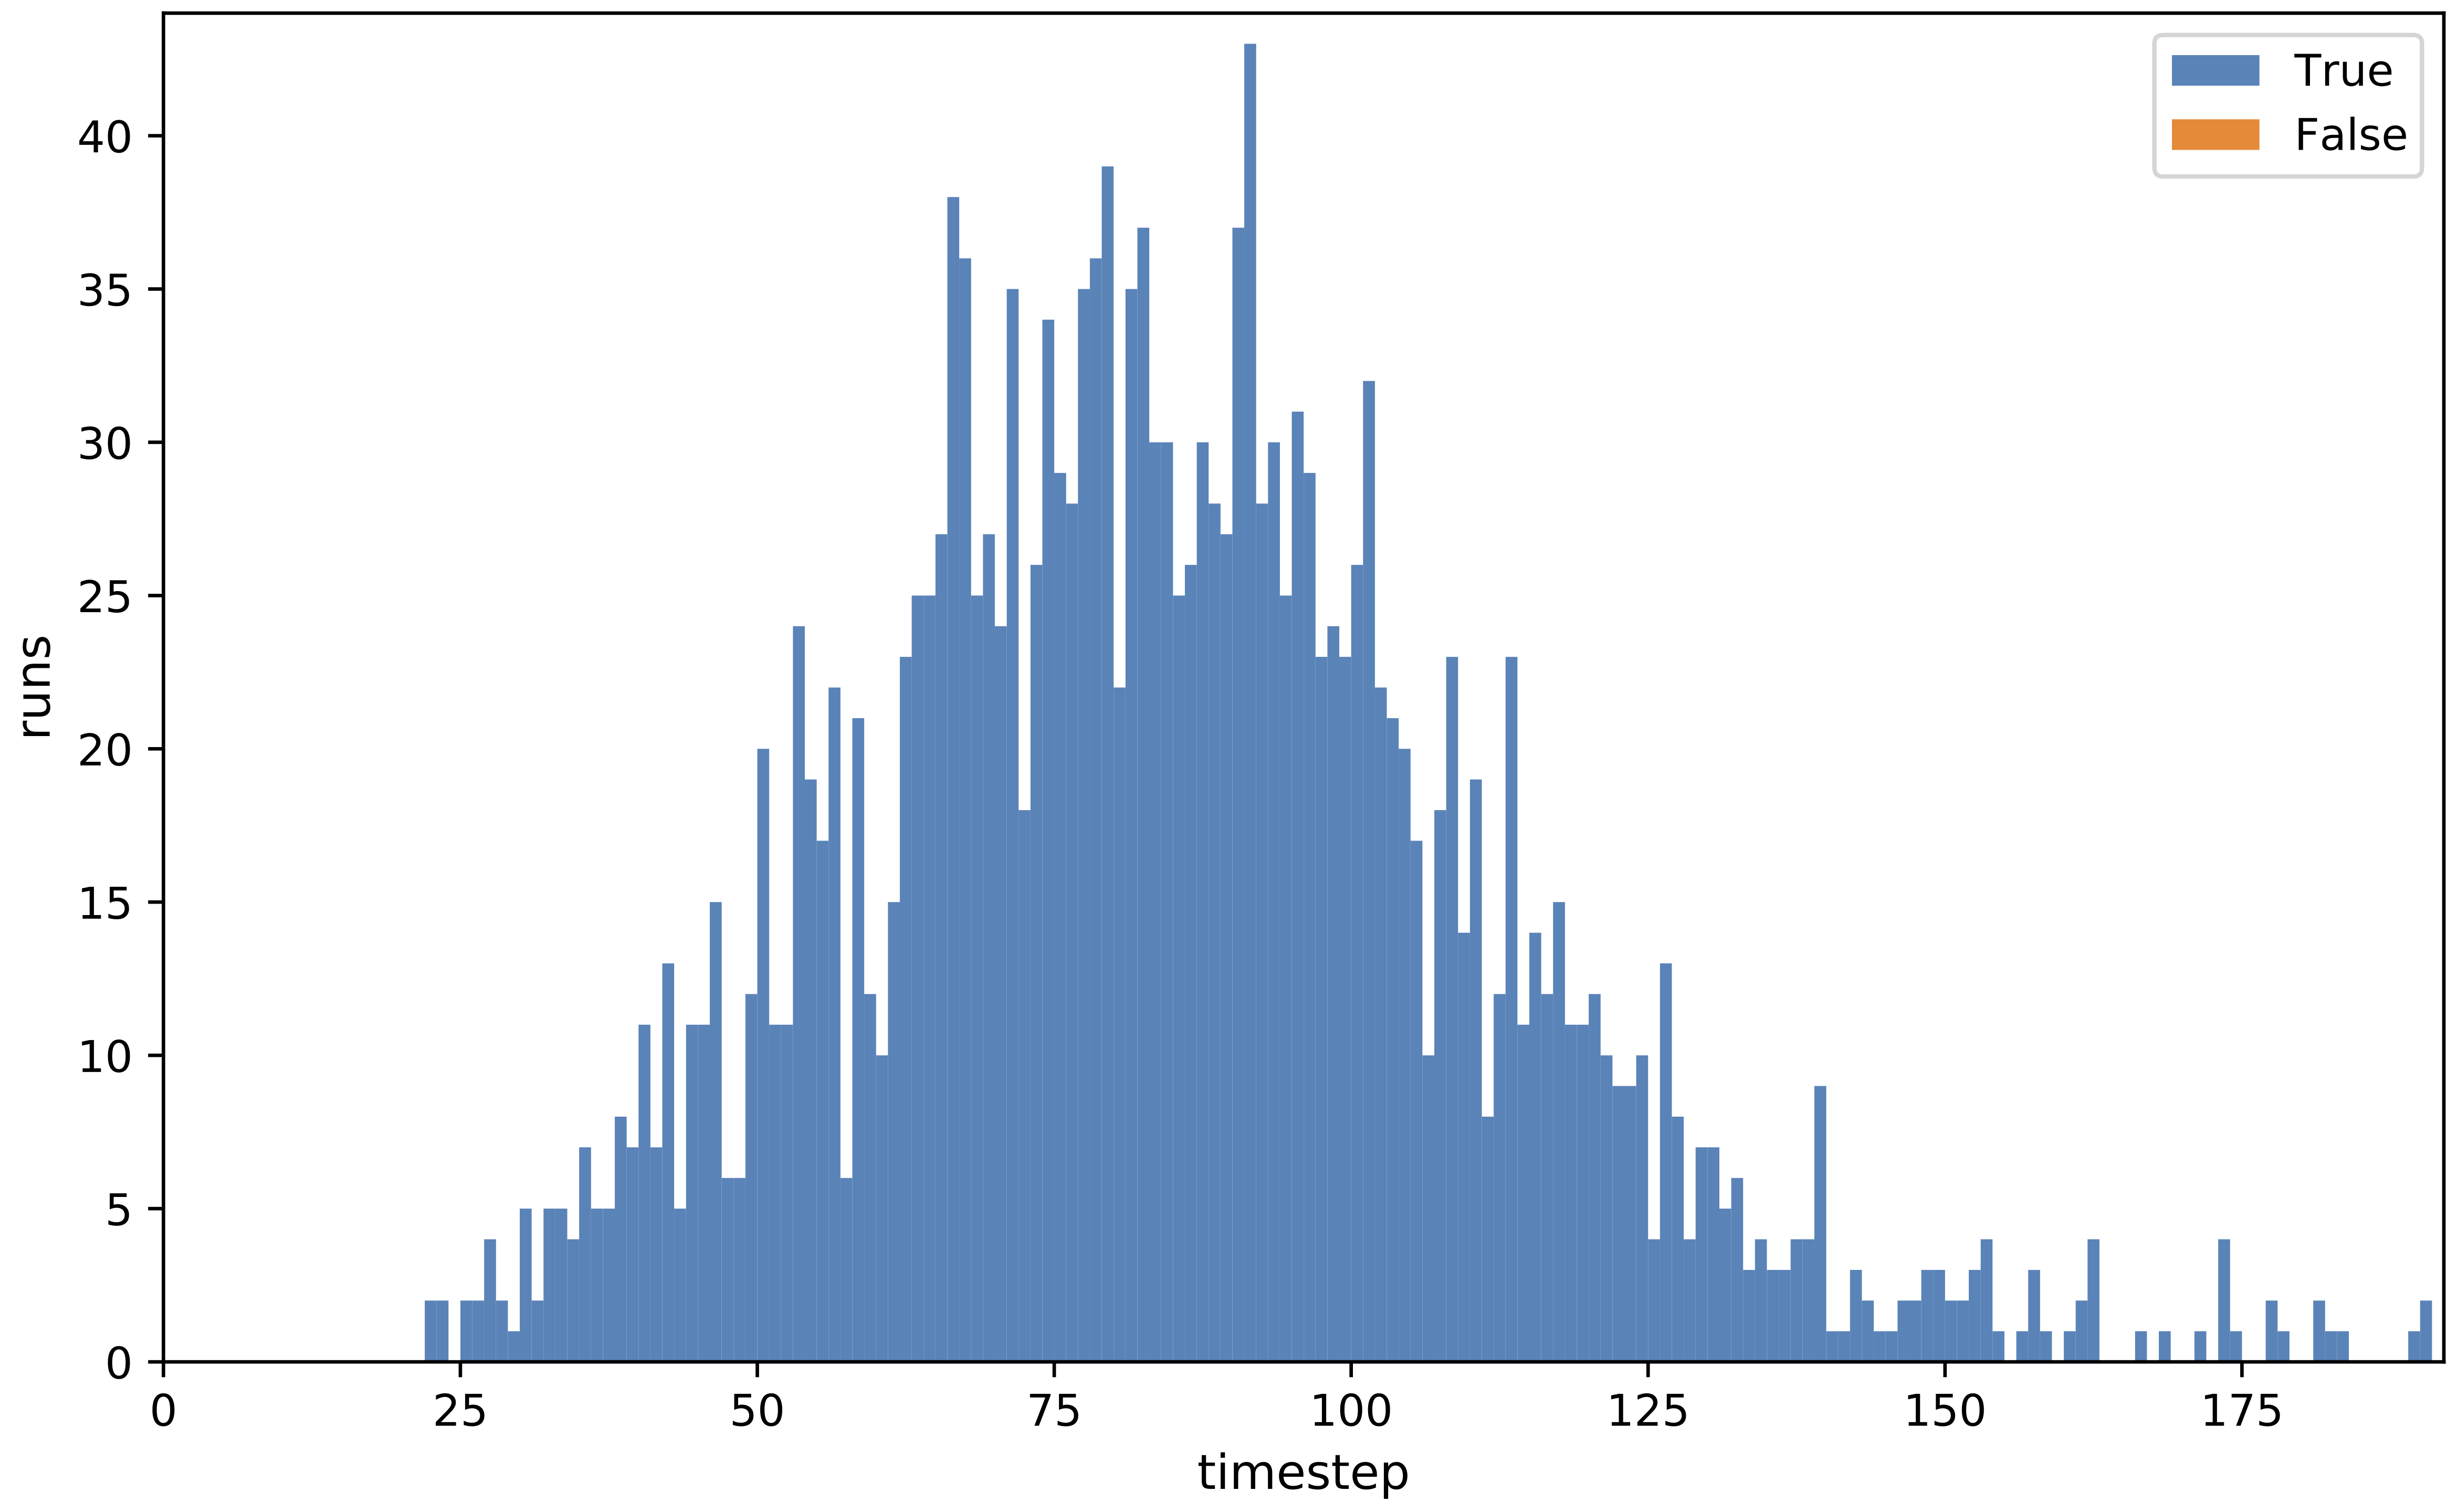
\includegraphics[width=.8\columnwidth]{dataset/monochromatic-omniscient/goal-reached}}
%	\caption{Time to reach the goal.}
%	\label{fig:goal-reached-omniscient}
%\end{figure}

Plotting the position and orientation errors over time shows the convergence of 
the omniscient controller. In Figure \ref{fig:distance-from-goal-omniscient} 
are shown the euclidean distance and the angular difference between the pose of 
the robot and the goal pose over time. In Figure \ref{fig:pose-over-time} is 
instead shown the pose over time.

%\begin{figure}[htbp]
%	
%\centerline{\includegraphics[width=\columnwidth]{dataset/monochromatic-omniscient/distances-from-goal}}
%	\caption{Distance from goal over time.}
%	\label{fig:distance-from-goal-omniscient}
%\end{figure}
%
%\begin{figure}[htbp]
%	
%\centerline{\includegraphics[width=.8\columnwidth]{dataset/monochromatic-omniscient/pose-over-time}}
%	\caption{Distance from goal over time.}
%	\label{fig:pose-over-time}
%\end{figure}

\section{Proposed Model}
The original dataset, that is the set of all the runs, is then shuffled and split, based on the single run, into the 
train, the validation and the test sets. The proportions are 70\% for training and 15\% each for validation and 
testing. In total, the training set is composed of 187000 samples.
The network trained is a CNN,  which takes as inputs the sensor distances and the camera image readings and as output 
produces the left and the right wheel target speeds. 
The input size is 180x4. The model is trained for 313 epochs, until early stopping interrupts it. 
The training set data are shuffled in each epoch, so the mini-batches (that are of size $2^14$) are generated 
independently. 
Adam is used as optimiser with learning rate $0.01$ and the loss function chosen is the Mean Squared Error (MSE). The 
other parameters have their default values. 
In the network the ReLU non-linearity is applied after every layer except the last one. 
The structure is the following:

\begin{table}[htbp]
	\caption{Architecture of the Baseline Network}
	\begin{center}
		\begin{tabular}{|c|c|c|c|c|}
			\hline
			\textbf{Layer}&\textbf{Channels} &\textbf{Kernel size} &\textbf{Stride} &\textbf{Padding}\\
			\cline{1-5}
			conv1 &  4 $\rightarrow$ 16 & 5 & 2 & 2, circular \\ \hline
			conv2 & 16 $\rightarrow$ 32 & 5 & 2 & 2, circular \\ \hline
			conv3 & 32 $\rightarrow$  			 32 & 5 & 1 & 2, circular \\ \hline
			fc1 &   45 $\times$ 32 $\rightarrow$ 128 &  &  &  \\ \hline
			fc2 &  128 $\rightarrow$ 128 &  &  &  \\ \hline
			fc3 &  128 $\rightarrow$   2 &  &  &  \\ \hline
		\end{tabular}
		\label{tab: baseline}
	\end{center}
\end{table}

\begin{table}[htbp]
	\caption{Architecture of the Network with Max Pooling}
	\begin{center}
		\begin{tabular}{|c|c|c|c|c|}
			\hline
			\textbf{Layer}&\textbf{Channels} &\textbf{Kernel size} &\textbf{Stride} &\textbf{Padding}\\
			\cline{1-5}
			conv1  &   4 $\rightarrow$  \bfseries	32 & 5 & 2 & 2, circular \\ \hline
			conv2  & \bfseries 32 $\rightarrow$  	96 & 5 & 2 & 2, circular \\ \hline
			\bfseries mpool1 & 					   & \bfseries 3	& \bfseries 3 & \bfseries 1, circular \\ 
			\hline			
			conv3  & \bfseries 96 $\rightarrow$  	96 & 5 & 1 & 2, circular \\ \hline
			fc1    & 15 $\times$ 96 $\rightarrow$ 128 &  &  &  \\ \hline
			fc2    & 128 $\rightarrow$ 128 &  &  &  \\ \hline
			fc3    & 128 $\rightarrow$   2 &  &  &  \\ \hline
			%\multicolumn{5}{l}{$^{\mathrm{a}}$Sample of a Table footnote.}
		\end{tabular}
		\label{tab: maxpool}
	\end{center}
\end{table}

\begin{table}[htbp]
	\caption{Architecture of the Network with Dropout}
	\begin{center}
		\begin{tabular}{|c|c|c|c|c|}
			\hline
			\textbf{Layer}&\textbf{Channels} &\textbf{Kernel size} &\textbf{Stride} &\textbf{Padding}\\
			\cline{1-5}
			\multicolumn{5}{|c|}{...} \\ \hline
			fc1 &  1440 $\rightarrow$ 128 &  &  &  \\ \hline
			\bfseries drop1 & \multicolumn{4}{c|}{\bfseries dropout with p = 0.5} \\ \hline
			fc2 &  128 $\rightarrow$ 128 &  &  &  \\ \hline
			\bfseries drop2 & \multicolumn{4}{c|}{\bfseries dropout with p = 0.5} \\ \hline
			fc3 &  128 $\rightarrow$   2 &  &  &  \\ \hline
			%\multicolumn{5}{l}{$^{\mathrm{a}}$Sample of a Table footnote.}
		\end{tabular}
		\label{tab: dropout + mpool}
	\end{center}
\end{table}



\begin{table}[htbp]
	\caption{Architecture of the Network for Task 2}
	\begin{center}
		\begin{tabular}{|c|c|c|c|c|}
			\hline
			\textbf{Layer}&\textbf{Channels} &\textbf{Kernel size} &\textbf{Stride} &\textbf{Padding}\\
			\cline{1-5}
			conv1  &  4 $\rightarrow$ 	32 & 5 & 2 & 2, circular \\ \hline
			conv2  & 32 $\rightarrow$  	96 & 5 & 2 & 2, circular \\ \hline
			mpool1 & 					   & 3	& 3 & 1, circular \\ 
			\hline			
			conv3  & 96 $\rightarrow$  	96 & 5 & 1 & 2, circular \\ \hline
			fc1   &  1440 \textbf{+ 3} $\rightarrow$ 128 &  &  &  \\ \hline
			drop1 & \multicolumn{4}{c|}{dropout with p = 0.5} \\ \hline
			fc2   &  128 $\rightarrow$ 128 &  &  &  \\ \hline
			 drop2 & \multicolumn{4}{c|}{ dropout with p = 0.5} \\ \hline
			fc3 &  128 $\rightarrow$   2 &  &  &  \\ \hline
			%\multicolumn{5}{l}{$^{\mathrm{a}}$Sample of a Table footnote.}
		\end{tabular}
		\label{tab: task 2}
	\end{center}
\end{table}


\subsection{Model performance}
%\begin{figure}[htbp]
%	\centerline{\includegraphics[width=.5\textwidth]{../models/net6/images/initial-positions.pdf}}
%	\caption{Initial positions divided by belonging dataset.}
%	\label{fig:initial-positions}
%\end{figure}
%
%\begin{figure}[htbp]
%	\centerline{\includegraphics[width=.5\textwidth]{../models/net6/images/loss.pdf}}
%	\caption{Comparison of the losses among the train and validation sets.}
%	\label{fig:loss}
%\end{figure}
%
%\begin{figure}[htbp]
%	\centerline{\includegraphics[width=.5\textwidth]{../models/net6/images/distribution-target.pdf}}
%	\caption{Comparison of the distributions of groundtruth and prediction of the validation set.}
%	\label{fig:distribution-target}
%\end{figure}
%
%\begin{figure}[htbp]
%	\centerline{\includegraphics[width=.5\textwidth]{../models/net6/images/regression.pdf}}
%	\caption{Comparison of the $R^2$regressor between groundtruth and prediction of the validation set.}
%	\label{fig:regression}
%\end{figure}

\subsection{Experiments}

%\begin{figure}[htbp]
%	\centerline{\includegraphics[width=.5\textwidth]{../models/net6/images/initial-positions.pdf}}
%	\caption{Initial positions divided by belonging dataset.}
%	\label{fig:initial-positions}
%\end{figure}
%
%\begin{figure}[htbp]
%	\centerline{\includegraphics[width=.5\textwidth]{../models/net6/images/loss.pdf}}
%	\caption{Comparison of the losses among the train and validation sets.}
%	\label{fig:loss}
%\end{figure}
%
%\begin{figure}[htbp]
%	\centerline{\includegraphics[width=.5\textwidth]{../models/net6/images/distribution-target.pdf}}
%	\caption{Comparison of the distributions of groundtruth and prediction of the validation set.}
%	\label{fig:distribution-target}
%\end{figure}
%
%\begin{figure}[htbp]
%	\centerline{\includegraphics[width=.5\textwidth]{../models/net6/images/regression.pdf}}
%	\caption{Comparison of the $R^2$regressor between groundtruth and prediction of the validation set.}
%	\label{fig:regression}
%\end{figure}


Using the learned controller, a new dataset has been generated, in which each run is stopped after 20 seconds, (maximum 
of 200 timesteps). 
In the following figures are shown some visualisation explaining the behavior of the robot controlled by the model.

\subsection{Results}
%\begin{figure}[htbp]
%	\centerline{\includegraphics[width=.5\textwidth]{../datasets/learned/images/10-robot-trajectories.pdf}}
%	\caption{Trajectories of ten randomly selected runs.}
%	\label{fig:trajectories-learned}
%\end{figure}
%
%\begin{figure}[htbp]
%	\centerline{\includegraphics[width=.5\textwidth]{../datasets/learned/images/positions-heatmap.pdf}}
%	\caption{Density of samples in each location.}
%	\label{fig:densisy-learned}
%\end{figure}
%
%\begin{figure}[htbp]
%	\centerline{\includegraphics[width=.5\textwidth]{../datasets/learned/images/distances-from-goal.pdf}}
%	\caption{Distance from goal over time.}
%	\label{fig:distance-from-goal-learned}
%\end{figure}
%
%\begin{figure}[htbp]
%	\centerline{\includegraphics[width=.5\textwidth]{../datasets/learned/images/goal-reached.pdf}}
%	\caption{Distribution of the reached goals over time.}
%	\label{fig:goal-reached-learned}
%\end{figure}
%
%\begin{figure}[htbp]
%	\centerline{\includegraphics[width=.5\textwidth]{../datasets/learned/images/initial-final-positions.pdf}}
%	\caption{Initial and final positions of the robot.}
%	\label{fig:initial-final-positions-learned}
%\end{figure}



\section{Task 2}

\begin{table}[htbp]
	\caption{Architecture of the Network for Task 2}
	\begin{center}
		\begin{tabular}{|c|c|c|c|c|}
			\hline
			\textbf{Layer}&\textbf{Channels} &\textbf{Kernel size} 
			&\textbf{Stride} &\textbf{Padding}\\
			\cline{1-5}
			conv1  &  4 $\rightarrow$ 	32 & 5 & 2 & 2, circular \\ \hline
			conv2  & 32 $\rightarrow$  	96 & 5 & 2 & 2, circular \\ \hline
			mpool1 & 					   & 3	& 3 & 1, circular \\ 
			\hline			
			conv3  & 96 $\rightarrow$  	96 & 5 & 1 & 2, circular \\ \hline
			fc1   &  1440 \textbf{+ 3} $\rightarrow$ 128 &  &  &  \\ \hline
			drop1 & \multicolumn{4}{c|}{dropout with p = 0.5} \\ \hline
			fc2   &  128 $\rightarrow$ 128 &  &  &  \\ \hline
			 drop2 & \multicolumn{4}{c|}{ dropout with p = 0.5} \\ \hline
			fc3 &  128 $\rightarrow$   2 &  &  &  \\ \hline
			%\multicolumn{5}{l}{$^{\mathrm{a}}$Sample of a Table footnote.}
		\end{tabular}
		\label{tab: task 2}
	\end{center}
\end{table}


\section{Future works/Problems/Solutions}
In task 2, it appears that the performance of the neural network is quite good 
at moving in the general direction of the goal, less so at arriving with the 
correct orientation or stopping at the right time.

The first issue should be mitigated by a bigger architecture and more training 
data, since at the moment we are using only 2000 runs as before, which might 
not be enough given the higher complexity of the task.

The reason for the second problem is that the omniscient controller never 
overshoots the goal, so the network does not see this situation in training.
In Task 1, we solved the same issue with a special case: we had the omniscient 
controller move in reverse when it spawns inside the arms of the object. A 
similar solution could be applied here, extending this trick to arbitrary goal 
poses.



%\section*{Acknowledgements}


\bibliographystyle{IEEEtran}
\bibliography{IEEEabrv, biblio}

\end{document}
